\documentclass[12pt]{article}
\usepackage[T1]{fontenc}
\usepackage[a4paper, total={7in, 10in}]{geometry}
\usepackage{graphicx}
\usepackage[export]{adjustbox}
\usepackage[font=normalsize,labelfont=bf]{caption}
\usepackage{caption}
\usepackage{subcaption}
\usepackage{float}
\usepackage{titling}
\usepackage{fancyhdr}
\usepackage{lipsum}
\newcommand{\mytitle}{Dynamiczny Eliminator Drgań}
\newcommand{\mysubtitle}{Modernizacja Stanowiska Pomiarowego}
\fancyfoot{}
\fancyhead[L]{\mytitle}
\fancyhead[R]{\mysubtitle}

\fancyfoot[C]{\thepage}


\renewcommand\maketitlehooka{\null\mbox{}\vfill}
\renewcommand\maketitlehookd{\vfill\null}
\renewcommand{\figurename}{Rysunek}
\graphicspath{{./tex_resources/}}
\title{\mytitle \\
  \large \mysubtitle}
\author{Mateusz Klisiewicz\thanks{Na podstawie \textit{Drgania mechaniczne – Laboratorium; Praca zbiorowa pod redakcją Z. Gałkowski; Oficyna Wydawnicza PW; 1999}}}
\date{\today}
\begin{document}
\pagestyle{fancy}
\maketitle
\newpage
\section*{Wstęp}
\subsection*{Obecna Postać Eksperymentu}
W obecnej postaci ćwiczenia studentom przedstawiana jest teoria tłumionego i nietłumionego dynamicznego eliminatora drgań, schemat stanowiska i niektóre parametry układu: $\mu$ - stosunek masy eliminatora do masy obudowy, $f$ - stosunek częstości eliminatora do częstości obudowy. \\Przeprowadza się dwa pomiary - pierwszy przy zblokowanym eliminatorze, drugi z odblokowanym eliminatorem. Do plików csv zapisywane są wartości przyspieszeń eliminatora i obudowy $a_1$, $a_2$, czas od rozpoczęcia pomiaru $t$  oraz częstotliwość wymuszenia bezwładnościowego $\nu$ . \\Następnie studenci sporządzają sprawozdanie, w którym zamieszczają krzywe rezonansowe przygotowane na podstawie zebranych danych i wnioski dotyczące porównania wyników doświadczalnych z teoretycznymi.
\subsection*{Problemy z Obecną Postacią Eksperymentu}
\subsubsection*{Teoria Dynamicznego Eliminatora Drgań}
Studentom przedstawia się instrukcję z teorią dynamicznego eliminatora drgań, która sporządzona jest na podstawie pierwotnej postaci stanowiska, w której rejestrowany był przebieg drgań na papierze przy użyciu długopisu połączonego z obudową układu. W efekcie studenci zbierali wykresy amplitud $A$ w zależności od częstotliwości wymuszenia ${\nu}$ i porównywali je z ich teoretycznymi wartościami, wyliczonymi na podstawie wzorów zawartych we wstępie teoretycznym. \\Współcześnie eksperyment opiera się na zbieraniu wartości przyspieszeń $a$, które są liniowo zależne od amplitud drgań $A$. Jednakże nie jest to sprecyzowane w instrukcji i niekoniecznie musi być oczywiste dla studentów wykonujących eksperyment.
\subsubsection*{Sposób Prowadzenia Pomiaru}
Układ wprawiany jest w drgania za pomocą wzbudnika, który jest niewyważoną masą obracaną przez silnik prądu stałego. Sterowanie częstotliwością wymuszenia polega na ręcznym kontrolowaniu napięcia zasilania silnika przy użyciu zasilacza laboratoryjnego. Obserwując wartość częstotliwości wymuszenia, zbieraną elektronicznie i wyświetlaną na ekranie komputera, koryguje się napięcie a następnie odczekuje się chwilę aby stan układu się ustalił. Taka metoda przede wszystkim wydłuża znacznie czas zbierania danych oraz wprowadza pewną niedokładność zebranych danych. Aplikacja stworzona na potrzeby eksperymentu zaczyna zbierać i wyświetlać dane w momencie kliknięcia przycisku "Rozpocznij pomiar", a więc w pliku odpowiadającym danej częstotliwości wymuszenia rejestrowany jest także czas, w którym stan układu nie został ustalony. \\Przy obróbce wyników konieczna jest korekcja otrzymanych wartości przyspieszenia $a$ o wartość przyspieszenia grawitacyjnego $g$. Sposób w jaki się tego dokonuje, a więc odjęcie średniej wartości przyspieszenia $a$ z danego pomiaru od uzyskanej maksymalnej wartości, wprowadza kolejne niedokładności. Metoda zbierania wartości $a$ z akcelerometrów przymocowanych do układu nie jest znana, natomiast korygując zebrane wartości zakłada się, że układ porusza się wyłącznie w osi $z$ prostopadłej do podłoża, co ponownie może choćby nieznacznie zaburzać wyniki.
\newpage
\subsubsection*{Niedoskonałości Układu i Aparatury Pomiarowej}
Na podstawie sprawozdania z ćwiczenia wykonanego 13.05.2024 (Załącznik nr 4) stwierdza się rozbieżność między informacjami zawartymi w instrukcji, a rzeczywistymi własnościami badanego układu. Widoczne jest istotne przesunięcie maksimum wyznaczonej krzywej rezonansowej układu z zablokwanym eliminatorem względem teoretycznego maksimum dla podanych wartości $\mu$ oraz $f$. Przesunięcie obserwuje się nawet po uwzględnieniu obliczonej wartości częstości drgań własnych obudowy układu $\omega_{10}$. Krzywa teoretyczna zdaje się pokrywać z krzywą eksperymentalną dopiero po założeniu $\omega_{10} = 17,75Hz$. \\Krzywa rezonansowa dla układu z odblokowanym eliminatorem odbiega w sposób istotny od przebiegu krzywej teoretycznej. Przede wszystkim zauważa się, znaczne przesunięcie względem $\frac{\nu}{\omega_{10}} = 1$ wynoszące w przybliżeniu $\Delta\nu =1,5Hz$. Wartość ta zdaje się pokrywać z rozdzielczością wykonywanych pomiarów. Ponadto, po uwzględnieniu tego przesunięcia, obserwuje się dużą rozbieżność w wartościach lokalnych maksimów w okolicach punktów charakterystycznych $P$ oraz $Q$, wyznaczona krzywa zdaje się być odbita względem prostej $\frac{\nu}{\omega_{10}} = 1$. Ponadto widoczna jest także duża różnica między wartościami zmierzonych przyspieszeń $a$ a ich wartościami teoretycznymi w zakresie $\frac{\nu}{\omega_{10}} > 1,2$.\\Po analizie teoretycznych zależności, przy założeniu $\mu = 0,05$  stwierdza się $f<1$ co może wyjaśniać niektóre rozbieżności i prowadzi do wniosku $\omega_{20} \ne \omega_{10}$, natomiast bez dokładnej inspekcji badanego układu ciężko jest jednoznacznie wyjaśnić te różnice, a studenta pozostawia się bez odpowiedzi.

\begin{figure}[H]
		\centering
		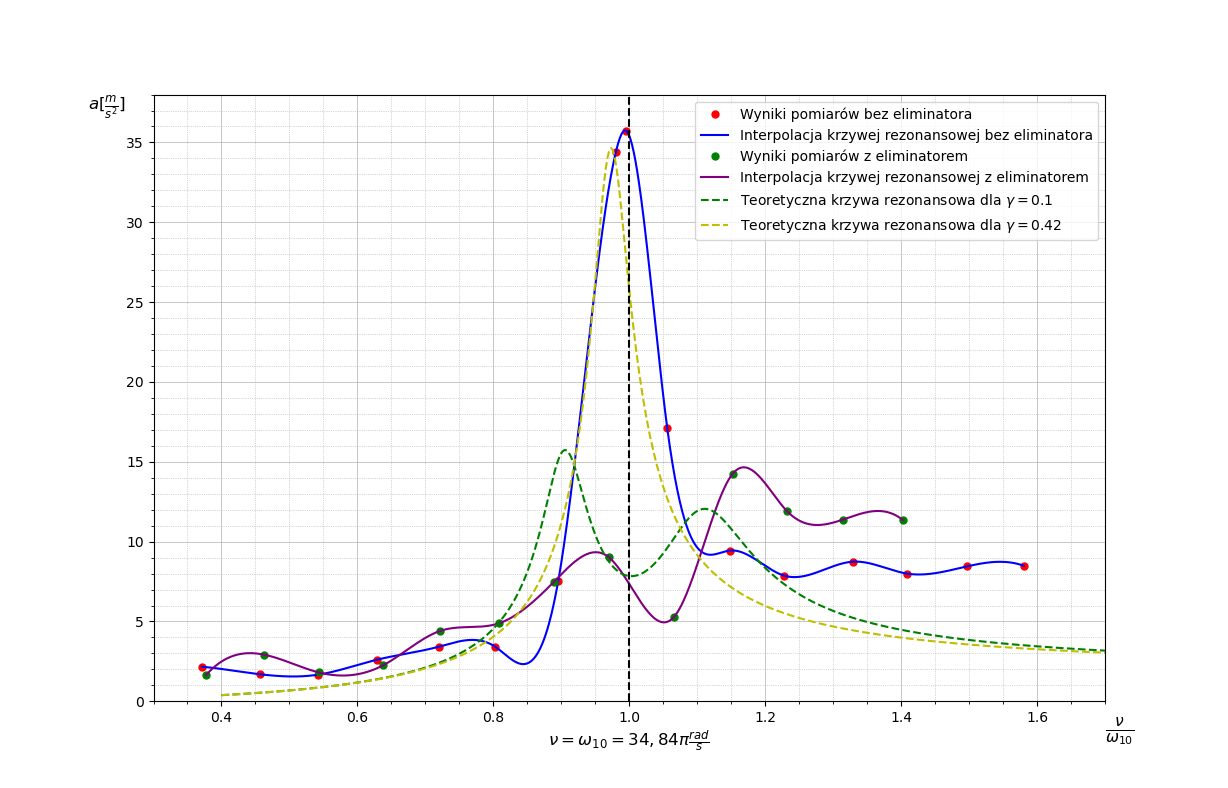
\includegraphics[width=\textwidth, left]{combination2}
		\caption{Wyznaczone krzywe rezonansowe po uwzględnieniu $\omega_{10}$ nałożone na krzywe teoretyczne}
		\label{rys:comb1}
\end{figure}

\begin{figure}[H]	
	\centering
	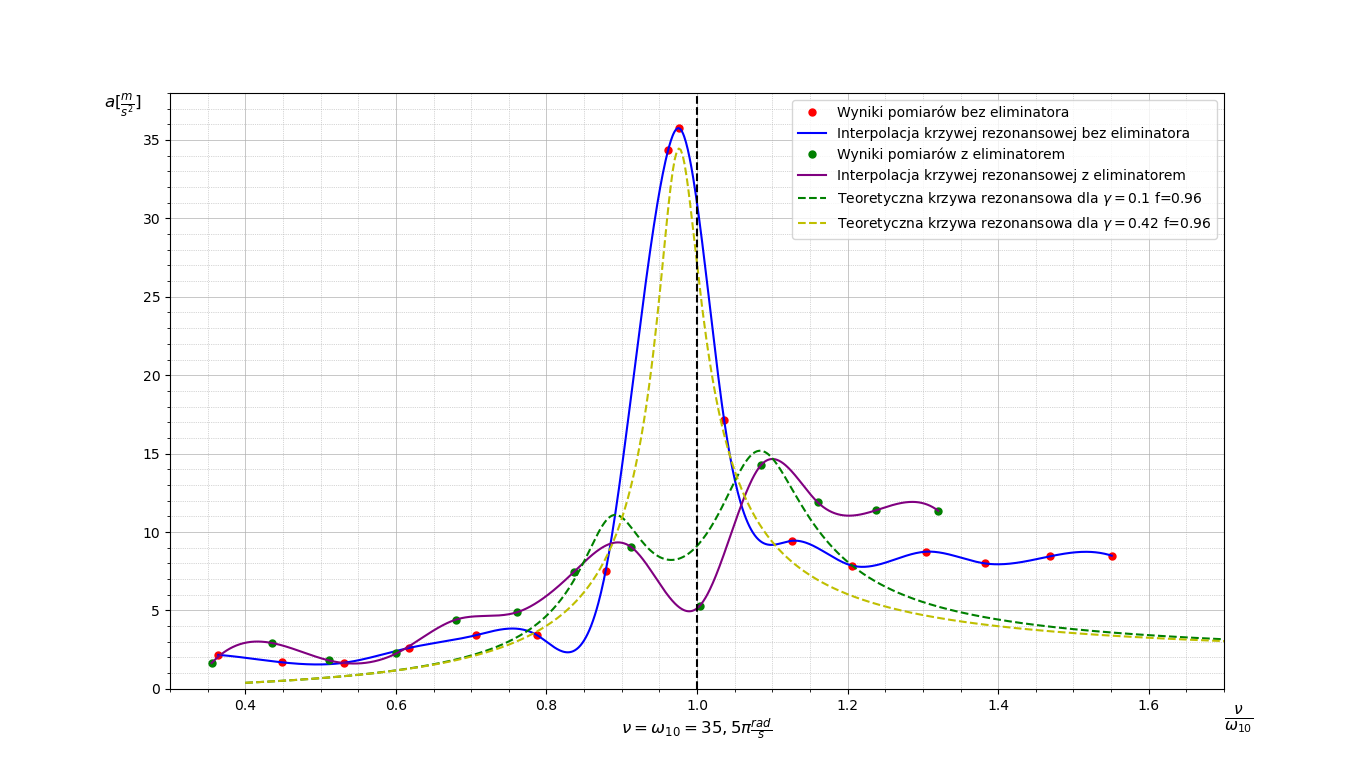
\includegraphics[width=\textwidth]{combination5}
	\caption{Wyznaczone krzywe rezonansowe po uwzględnieniu przesunięcia, $\omega_{10}=17,75Hz$ oraz $f\approx0,96$ nałożone na krzywe teoretyczne}
	\label{rys:comb2}
\end{figure}

\section*{Propozycja Modyfikacji Eksperymentu}
Adresując wyżej opisane problemy proponuje się następującą modyfikację eksperymentu:
\subsection*{Modyfikacja Wprowadzenia Teoretycznego}
Biorąc pod uwagę fakt mierzenia przyspieszeń obudowy, należałoby odpowiednio poprawić instrukcję do ćwiczenia podając zależność amplitudy drgań od przyspieszenia lub bezpośrednio operując na przyspieszeniach układu.
\subsection*{Zmiana Sposobu Przeprowadzania Pomiarów}
Chcąc wykluczyć niedokładności powodowane ręcznym sterowaniem zasilania, modyfikuje się układ elektroniczny tak by kontroler stanowiska zasilany był z zasilacza 24VDC, zgodnie ze schematem (Rys. 3). Odpowiednio modyfikując oprogramowanie mikrokontrolera uzyskuje się możliwość automatycznego ustalania częstotliwości wymuszenia, według zadanych parametrów. Skraca się także czas potrzebny na wykonanie jednego pomiaru w zadanym zakresie częstości, co umożliwia wykonanie eksperymentu kilkukrotnie w trakcie jednych zajęć.
Zaproponowany program laboratoryjny po podaniu parametrów $\mu$, $f$ umożliwiałby ustalenie zakresu badanych częstości oraz rozdzielczości pomiaru, wykonywałby eksperyment, a następnie na podstawie wyników rysował wykresy eksperymentalnych i teoretycznych krzywych rezonansowych gotowych do analizy przez studentów.

\begin{figure}[H]
	\centering
	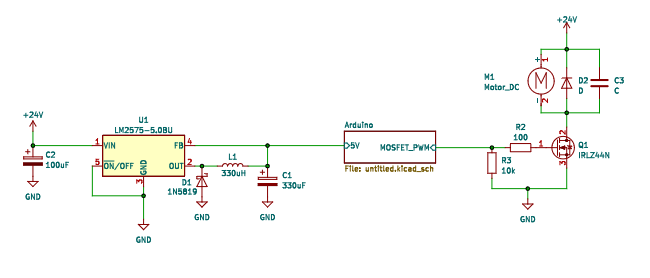
\includegraphics[width=0.75\textwidth]{dem_sch}
	\caption{Schemat zasilania mikrokontrolera}
	\label{fig:sch}
\end{figure}

\subsection*{Inspekcja Stanowiska Badawczego}
Zauważając nieprawidłowości w wynikach eksperymentów, należałoby dokonać inspekcji układu, sprawdzić faktyczne masy obudowy i eliminatora, wyznaczyć rzeczywiste częstości drgań własnych oraz parametry $f, \mu, \gamma$. Przyjrzeć się sposobowi zbierania wartości przyspieszeń i ewentualnie uwzględnić zmiany pozycji akcelerometru w osi poziomej.

\subsection*{Zmiana Celu Ćwiczenia}
Program laboratoryjny umożliwiłby automatyczne rysowanie krzywych rezonansowych, co pozwala szybko przygotować teoretyczne wykresy dla zadanych wartości $\gamma, \mu, f$. Dzięki temu łatwo jest zwizualizować teoretyczną zależność krzywej rezonansowej od tych parametrów. Z tego powodu można zmienić cel ćwiczenia, który obecnie polega na wysnuciu wniosków na podstawie sporządzonych krzywych. Proponuje się aby studenci otrzymali wartość masy obudowy $M$, sztywność sprężyn obudowy $K$ i na tej podstawie odszukali częstość drgań własnych $\omega_{01}$, a następnie dokonali "strojenia" eliminatora odszukując pożądane $\gamma, \mu, f$. Otrzymane wyniki wpisaliby do aplikacji aby otrzymać teoretyczne krzywe rezonansowe, które następnie porównaliby z krzywymi otrzymanymi w wyniku eksperymentu. Jeżeli zaobserwuje się istotne różnice, studenci mieliby za zadanie znaleźć przyczyny tych rozbieżności, manipulując parametrami aż do otrzymania poprawnych wyników. Ostatecznie sposób postępowania byłby relacjonowany w sprawozdaniu zdawanym prowadzącemu zajęcia.
\section*{Podsumowanie}
Opisane wyżej modyfikacje, wykorzystujące możliwości nowoczesnych urządzeń elektronicznych, niewielkim kosztem, pozwoliłyby studentom na doświadczenie pracy laboratoryjnej na miarę XXI wieku. Jasno postawiony cel eksperymentu zwiększyłby zaangażowanie, a jednoznaczne rozwiązanie problemu przedstawiłoby różnice między teoretycznymi rozważaniami i ich praktycznym zastosowaniem.
\end{document}